
\documentclass[a4paper,10pt]{article}
\usepackage[utf8]{inputenc}
\usepackage[T1]{fontenc}
\usepackage[left=0.8cm,right=0.8cm,top=0.8cm,bottom=0.8cm]{geometry}
\usepackage{enumitem}
\usepackage{titlesec}
\usepackage{parskip}
\usepackage{graphicx}
\usepackage{hyperref}
\usepackage{tikz}
\usepackage{adjustbox}
\usepackage{xcolor}
\usepackage[most]{tcolorbox}
\usepackage{pifont}
\definecolor{bleu}{HTML}{013c63}
\newcommand{\starfull}{\textcolor{bleu}{\ding{72}}}
\newcommand{\starempty}{\textcolor{bleu}{\ding{73}}}
\newcommand{\starhalf}{\textcolor{bleu}{\ding{74}}}
\newcommand{\cvtext}{\fontsize{8}{10}\selectfont}
\newcommand{\cvtextsmall}{\fontsize{7}{9}\selectfont}
\tcbset{
  cvbox/.style={
    colframe=bleu,
    colback=white,
    boxrule=0.4pt,
    arc=2pt,
    left=6pt,
    right=6pt,
    top=4pt,
    bottom=4pt,
    enhanced
  }
}
\titleformat{\section}{\Large\bfseries\color{bleu}}{}{0em}{}[\vspace{-0.5em}]
\titleformat{\subsection}{\bfseries\color{bleu}}{}{0em}{}[\vspace{-0.3em}]
\pagestyle{empty}
\hypersetup{
  pdfauthor={Victor Dauphin},
  pdftitle={CV Victor Dauphin},
  pdfsubject={CV},
  pdfproducer={LaTeX},
  pdfcreator={pdflatex},
  colorlinks=true,
  urlcolor=bleu,
  linkcolor=bleu,
  citecolor=bleu
}
\begin{document}
\noindent
\begin{minipage}[t]{0.72\textwidth}
  {\LARGE \textcolor{bleu}{\textbf{Technical Mentor - Développeur Fullstack Java / Angular}}}\\[0.5em]
  {\LARGE \textcolor{bleu}{\textbf{Victor Dauphin}}}\\[0.5em]
  Metz • 37 ans • Permis B \\
  \href{mailto:victor.dauph@gmail.com}{victor.dauph@gmail.com} • +33 6 95 19 99 40 \\
  \href{https://github.com/VictorDauph}{GitHub} •
  \href{https://linkedin.com/in/victor-dauphin-83430840}{LinkedIn}\\
\end{minipage}
\hfill
\begin{minipage}[t]{0.25\textwidth}
  \begin{flushright}
  \raisebox{-2.6cm}{
    \begin{tikzpicture}
      \draw[fill=white, draw=bleu, line width=1pt] (0,0) circle (1.51cm);
      \clip (0,0) circle (1.5cm);
      \node at (0,0) {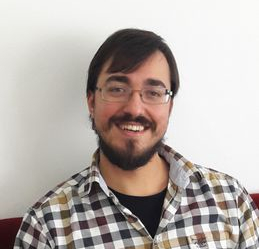
\includegraphics[width=3cm]{images/photo.jpg}};
    \end{tikzpicture}
    }
  \end{flushright}
\end{minipage}
\vspace{0.8em}
\noindent
\begin{minipage}[t]{0.3\textwidth}
  \section*{Compétences}
  \begin{tcolorbox}[cvbox, width=\linewidth]
      \subsection*{Stack Principale}
      {\normalsize
      Java / Spring Boot \\
      Angular / Typescript \\
      PostgreSQL
      } \\
      \subsection*{Technologies Complémentaires}
      {\normalsize
      Node.js / Express / NestJS \\
      Vue.js \\
      MongoDB \\
      NiFi \\
      PHP / Dolibarr
      } \\
      \subsection*{Devops \& Quality}
      {\normalsize
      Docker \\
      Gitlab CI \\
      Tests unitaires : JUnit \\
      SonarQube / ESLint
      } \\
      \subsection*{Bonnes pratiques}
      {\normalsize
      Clean Code \\
      SOLID \\
      CI/CD \\
      OWASP \\
      WCAG \\
      Git workflow
      }
  \end{tcolorbox}
  \section*{Certifications}
  \begin{tcolorbox}[cvbox, width=\linewidth]
    \begin{itemize}[leftmargin=*]
      \item AWS Cloud Practitioner (2023)
      \item DevSecOps Foundation (2023)
      \item 2AIConcept Expert Trainer (2024)
    \end{itemize}
  \end{tcolorbox}
  \section*{Diplômes}
  \begin{tcolorbox}[cvbox, width=\linewidth]
    \begin{itemize}[leftmargin=*]
      \item M2i \textit{POEI Fullstack Spring/Angular} (2022)
      \item OpenClassrooms \textit{Fullstack Node/React} (2021)
      \item ENSGSI \textit{Ingénieur généraliste} (2013)
    \end{itemize}
  \end{tcolorbox}
\end{minipage}
\hfill
\begin{minipage}[t]{0.68\textwidth}
\section*{Profil}
  Développeur Fullstack Java / Angular avec 4 ans d’expérience en environnement entreprise.
Je conçois des applications robustes en mettant l’accent sur la qualité du code, le CI/CD et les bonnes pratiques d’ingénierie.
J’accompagne également les équipes dans la structuration des projets et la montée en compétence technique.\\
\section*{Expériences professionnelles}
\begin{tcolorbox}[cvbox, width=\linewidth, fontupper=\cvtext]
    \subsection*{Formateur en développement Web -- freelance} \textit{Oct 2024 -- Aujourd'hui}
    \begin{itemize}[leftmargin=*]
      \item Les nouveautés de Java (v6 à v21).
      \item HTML et CSS modernes
      \item Angular : architecture, composants, services, RxJS, Reactive Forms.
      \item Initiation SQL/PostgreSQL.
      \item PL/SQL: procédures stockées, fonctions, triggers dans une base de données Oracle.
    \end{itemize}
    \subsection*{Développeur freelance -- Arterrien \textit{PHP / Dolibarr}} \textit{Avr 2025 -- Juin 2025}
    \begin{itemize}[leftmargin=*]
      \item Maintenance évolutive d’un module ERP basé sur Dolibarr.
      \item Mise en place de PHPStan (niveau 4) avec stubs personnalisés pour le contexte Dolibarr.
      \item Création d’un runner CI/CD Dockerisé (Google Cloud VM + GitLab).
      \item Implémentation de tests unitaires avec PHPUnit.
    \end{itemize}
    \subsection*{Formateur CDA \textit{Express / Angular}} \textit{Nov 2024 -- Avr 2025}
    \begin{itemize}[leftmargin=*]
      \item Formation intensive pour demandeurs d’emploi.
      \item Projets pratiques : Angular, Express, MongoDB, SQL.
      \item Docker, Git, CI/CD, tests automatisés.
    \end{itemize}
    \subsection*{Développeur Fullstack -- Davidson \textit{Vue / NestJS}} \textit{Juin 2024 -- Sept 2024}
    \begin{itemize}[leftmargin=*]
      \item Refonte du Vue Router, mise en place des modules todo/notifications.
      \item Peer reviews, documentation, mise en production.
    \end{itemize}
    \subsection*{Développeur Nifi / Java -- Atos / EDF \textit{NiFi / Java / VBA}} \textit{Sept 2023 -- Juin 2024}
    \begin{itemize}[leftmargin=*]
      \item Conception et développement de flux de données avec Apache NiFi.
      \item Création d’un processeur NiFi personnalisé en Java pour répondre à des besoins métiers spécifiques.
      \item Automatisation de tâches avec des macros Excel (VBA) et rédaction de tests avec Unifier.
    \end{itemize}
    \subsection*{Développeur Fullstack -- Atos /  Agirc-Arrco / CEA \textit{Angular / Java SpringBoot}} \textit{Octobre 2022 -- Juin 2023}
    \begin{itemize}[leftmargin=*]
      \item Développement d’interfaces utilisateurs en Angular, intégrées à des APIs REST.
      \item Conception de services backend avec Spring Boot et gestion des données via PostgreSQL.
      \item Rédaction de tests unitaires avec JUnit pour garantir la fiabilité du code.
      \item Implication dans tout le cycle projet : analyse, développement, tests, et livraison en environnement agile.
    \end{itemize}
\end{tcolorbox}
\section*{Autres expériences professionnelles}
\begin{tcolorbox}[cvbox, width=\linewidth, fontupper=\cvtextsmall]
  \begin{itemize}[leftmargin=*]
    \item \textbf{Formateur indépendant} – Communication interpersonnelle (2018–2020)  
    Animation de formations dynamiques basées sur le théâtre d’improvisation.

    \item \textbf{Chargé de mission} – Logistique durable (2017–2018)  
    Promotion de solutions écoresponsables dans un cluster logistique.

    \item \textbf{Chef de projet} – Logistique médicale (2016–2017)  
    Coordination d’équipes et gestion de flux pour la recherche clinique.

    \item \textbf{Co-fondateur} – Startup numérique (2013–2015)  
    Développement produit, management d’équipe, stratégie commerciale.
  \end{itemize}
\end{tcolorbox}

\end{minipage}
\end{document}
